\section{Linkability and Unlinkability}
\label{sec:unlinkability}

All CC Protocols discussed so far provide retailers with a property of credit card payments known as \emph{linkability}:
    retailers are able to link distinct purchases that are made using the same credit card, in order to build purchasing profiles on their customers.
Customer purchasing profiles are valuable to retailers, because they allow for more targeted and effective marketing, and can be sold to interested third parties.

Recall that in the Insecure CC Protocol described in Chapter \ref{cha:insecure} (and in widespread use today),
  the credit card discloses its card number, expiration date, and iCVV to the point of sale with every purchase.
Therefore, a retailer can link purchases that are made by the same credit card simply by comparing the card numbers of these purchases.
Note that any credit card protocol which gives the retailer access to the card number is linkable by definition.

These purchasing profiles can be unpleasant to the customer from a privacy standpoint:
  purchasing habits can reveal sensitive and personal information.
Furthermore, a customer cannot opt-out of this profiling except by avoiding the use of credit cards altogether.

With this in mind, we consider how to provide credit card payments with the converse property: \emph{unlinkability}.
Informally, if credit card purchases are unlinkable, then retailers cannot use them to construct purchasing profiles efficiently.

While giving the retailer access to the card number is sufficient to undermine unlinkability, it is not necessary.
For example, consider the Secure CC Protocol, presented in Chapter \ref{cha:secure} and shown in Figure \ref{fig:secure_ccp_recall} for convenience.
In this protocol, the credit card number is not disclosed, and all authentication data (contained within the value \emph{T}) is indistinguishable from random to the retailer.
However, the charge token contains a constant card identifier \emph{ID}, required by the bank in order to identify the customer for which \emph{T} must be verified.
No two credit cards have the same \emph{ID}, and \emph{ID} does not change, so the retailer can simply link purchases using \emph{ID} instead of the card number.
More generally, if the protocol includes a message received by the retailer from which the customer's identity can be inferred, then the protocol cannot provide unlinkability.

\begin{figure}[h!]
  \caption{Secure CC Protocol}
  \centering
    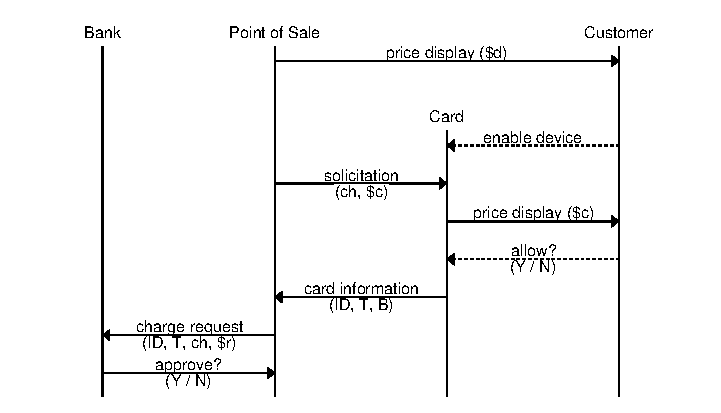
\includegraphics{img/secure_ccp.eps}
  \label{fig:secure_ccp_recall}
\end{figure}


While we wish to conceal the customer's identity from the retailer, it must be disclosed to the bank in order for a charge to be processed.
As such, the problem reduces to one where we wish the contents of a message generated by a credit card (the message source)
  to be opaque to the point of sale (the carrier), but not to the bank (the final destination).
A natural approach to this problem is to use cryptography.
